%%%%%%%%%%%%%%%%%%%%%%%%%%%%%%%%%%%%%%%%%
% Chemical Equations
% LaTeX Template
% Version 1.0 (14/10/12)
%
% This template has been downloaded from:
% http://www.LaTeXTemplates.com
%
% Original author:
% Martin Hensel (from the mhchem package documentation)
%
% License:
% CC BY-NC-SA 3.0 (http://creativecommons.org/licenses/by-nc-sa/3.0/)
%
% Note: to use these chemistry equations in your own document you will
% need to copy the \usepackage[version=3]{mhchem} line and paste it 
% before \begin{document} in your document. After this you can use the
% chemistry equation notation as exemplified in this document anywhere
% in your document.
%
%%%%%%%%%%%%%%%%%%%%%%%%%%%%%%%%%%%%%%%%%

\documentclass{article}

\usepackage[version=3]{mhchem} % Package for chemical equation typesetting
\usepackage{amsmath}
\usepackage[makeroom]{cancel}
\usepackage{physics}
\usepackage{tikz}
\usetikzlibrary{calc,scopes,angles,quotes,positioning}
\usepackage[portuges]{babel}
\usepackage{pdfpages}
%\usetikzlibrary{scopes}
\usepackage[utf8]{inputenc} % usually not needed (loaded by default)
\usepackage[T1]{fontenc}

\begin{document}
\everymath{\displaystyle}
\def\iangle{30} % Angle of the inclined plane

\def\down{-90}
\def\arcr{0.5cm} % Radius of the arc used to indicate angles


%									2a
\paragraph{2a)} ~\\
\begin{center}
\begin{tikzpicture}[
    force/.style={>=latex,draw=blue,fill=blue},
    axis/.style={densely dashed,gray,font=\small},
    aux/.style={draw=gray,font=\small},
    M/.style={circle,draw,fill=lightgray,minimum size=0.7cm,thin},
    m/.style={rectangle,draw=black,fill=lightgray,minimum size=0.3cm,thin},
    plane/.style={draw=black,fill=blue!10},
    string/.style={draw=red, thick},
    pulley/.style={thick},
    tubo/.style={thick,draw=gray},
]


    \begin{scope}[rotate=\iangle]
        \node [M,transform shape] (M) {$M$};
        % Draw axes and help lines

        {[axis,->]
           % \draw (0,-1) -- (0,2) node[right] {$+y$};
            \draw (2,0) -- (-2,0) node[left] {$+x$};
            % Indicate angle. The code is a bit awkward.

        }
	{[plane]
	\draw (-2,-0.4) -- (2,-0.4);
	}
        % Forces
        {[force,->]
            % Assuming that Mg = 1. The normal force will therefore be cos(alpha)
            \draw (M.center) -- ++(0,{cos(\iangle)}) node[above right] {$Rn$};
            \draw (M.west) --(-2*sin{\iangle},0) coordinate (ft) node [left] {$F_{gtan}$};
            \draw (M.south) -- ++ (1,0) node [above] {$F_a$};
           % \draw (M.east) -- ++(1,0) node[above] {$T$};
        }
        

    \end{scope}
    % Draw gravity force. The code is put outside the rotated
    % scope for simplicity. No need to do any angle calculations. 
    \draw[force,->] (M.center) -- ++(0,-2) coordinate (fg) node [below right=-0.15cm] {$F_g$};
    {[aux]
	\draw (0,-1.5) arc (90:90+\iangle:0.5);
	\node at (-0.2,-1.3) {$\theta$};
	}
    \draw[axis] (ft) -- (fg);

\end{tikzpicture}
\end{center}
$
m=0,2kg  \quad \theta = 30^\circ \quad r=0.05m\\
F_g=mg\\
F_{gtan}=F_g \sin(\theta)=mg\sin(\theta)\\
\\
$Bola roda sem deslizamento$ \quad \Rightarrow v_{cm}=\omega r
\\
\\
\dv{L}{t}=T=rF_a  \quad \wedge \quad \dv{L}{t}=I\dot \omega=I \frac {a_{cm}}{r}\\
\Leftrightarrow F_a=I \frac{a_{cm}}{r^2}\\
\\
\dv{P}{t}=ma=\Sigma F=F_{gtan}-F_a=mg\sin{\theta}-I \frac{a}{r^2}\\
\\
\cancel{m}a=\cancel{m}g\sin\theta-\frac{2}{5}\cancel{m}\bcancel{r^2}\frac{a}{\bcancel{r^2}}
\\
\Leftrightarrow \boxed{a=\frac{5}{7}g\sin(\theta)=3.5rad/s^{2}}\\
\\
%Alternativamente:\\
%\Delta T=\Delta V
%\Leftrightarrow mgh=\frac{1}{2}mv^2 \Leftrightarrow v=\sqrt{2gh}\\
%\\
%v=at \Leftrightarrow t=\frac{\sqrt{2gh}}{g\sin(\phi)}
$
%
%$V=-mgl \cos (\theta)$\\
%\\
%$T=\frac{1}{2}mv^{2}=\frac{1}{2}ml^2 \dot \theta^2$\\
%\\
%\boxed{L=\frac{1}{2}ml^2 \dot \theta^2+mgl \cos (\theta)}\\
%\\
%$
%\Rightarrow \frac{d}{dt} (ml^2 \dot \theta)=-mgl \sin (\theta)\\
%\\
%\Leftrightarrow \ddot \theta=-\frac{g}{l}\sin(\theta)$\\
%\\
%Para pequenos ângulos $\sin(\theta)\approx\theta\\
%\\
%\Rightarrow \ddot \theta=-\frac{g}{l}\theta \\
%\\\draw [aux,->](-1.5,1) arc (-70:-110:1) arc(250:110:0.05) arc (110:80:1);
%\Leftrightarrow \theta=\sin(-\sqrt{\frac{g}{l}}t) \qquad \theta(t)=\sin(-\omega t)
%$

%
%$v_k=\frac{\partial r_k}{\partial q_j}\dot q_j + \cancel{\frac{\partial r_k}{\partial t}}$\\
%\\
%$r(q,t)=(l\sin(\theta),l\cos(\theta))$\\
%\\
%$v=(l\dot \theta \cos(\theta), -l \dot \theta \sin(\theta)$
%
%$v^2=l^2 \dot \theta^2 \cancelto{1}{(\cos^2(\theta)+\sin^2(\theta))}$\\
%\\\draw [aux,->](-1.5,1) arc (-70:-110:1) arc(250:110:0.05) arc (110:80:1);
%\\
%\\ \\ \\ \\ \\
%\boxed{\omega=\sqrt{\frac{g}{l}}}
\hrule
%%%%%%%%%%%%%%%%%%%%                     2b
\paragraph{2b)} ~\\
\\
$
V_{i}=mgh \quad T_i=0 \quad \wedge \quad V_f=0 \quad T_f=\frac{1}{2}mv^2+\frac{1}{2}I\omega^2\\
$Roda sem deslizamento$\quad \Rightarrow v_{cm}=\omega r\\
\\
\Leftrightarrow \cancel{m}gh=\frac{1}{2}\cancel{m}v^2+\frac{1}{5}\cancel{m}v^2\\
\\
\boxed{v=\sqrt{\frac{10gh}{7}}=5.29m/s}\\
$
%2 graus de liberdade: $\theta$ e x\\
%\\
%$
%r_m=(x+l\sin(\theta),-l\cos(\theta)) \quad v_m=(\dot x+l\dot \theta \cos(\theta),l\dot \theta \sin(\theta)) \\
%\\
%v^2_m=(\dot x+l\dot \theta \cos(\theta))^2+(l\dot \theta \sin(\theta))^2=\dot x^2+2+\dot x+\dot \theta \cos(\theta)+l^2 \dot \theta^2 \cancelto{1}{(\cos^2(\theta)+\sin^2(\theta))}\\
%\\
%r_M=(x,cte) \quad v_M=\frac{\partial r_k}{\partial q_j} \dot q_j = (\dot x, 0) \qquad v^2_M=\dot x^2$ \\
%\\
%
%\boxed{L=\frac{M \dot x^2}{2}+\frac{m \dot x^2}{2}+m \dot xl \dot \theta \cos\theta+\frac{ml^2 \dot \theta^2}{2}+mgl\cos\theta}\\
\\
\hrule
 \pagebreak
%									2c
\paragraph{2 c)} ~\\
Colisão elástica
\\
$
\Delta \vec{P}=0 \quad \wedge \quad \Delta \vec{E_c}=0\\
mv_{Ai}+\cancel{mv_{Bi}}=mv_{Af}+mv_{Bf}\Leftrightarrow \boxed{v_{Bf}=v_{Ai}-v_{Af}}\\ 
\frac{1}{2}mv_{Ai}^2+\cancel{\frac{1}{2}mv_{Bi}^2}=\frac{1}{2}mv_{Af}^2+\frac{1}{2}mv_{Bf}^2\\
\\
$
Substituindo com $v_{Bf}=v_{Ai}-v_{Af}\\
\frac{1}{2}mv_{Ai}^2=\frac{1}{2}m(v_{Af}-v_{Ai})^2+\frac{1}{2}mv_{Af}^2\\
\\
\Leftrightarrow v_{Af}v_{Ai}=v_{Af}^2
\Leftrightarrow \left \{
\begin{aligned}
v_{Af}&=0\\
v_{Bf}&=v_{Ai}\\
\end{aligned}
\right . 
\lor \left \{
\begin{aligned}
v_{Af}&=v_{Ai}\\
v_{Bf}&=0\\
\end{aligned}
\right . 
\\
\\
$Como a bola B está na frente de A, $v_{Af}=0 \land v_{Bf}=v_{1i}\\
$Como não existe atrito entre as bolas, não existe transferência de momento angular da bola 1 para a bola 2 e $\omega_{Ai}=\omega_{Af} \land \omega_{Bi}=\omega_{Bf}=0\\
$
%\dv{t} (\pdv{L}{\dot x})=$\boxed{M \ddot x + m \ddot x +ml\ddot \phi \cos \theta - ml\dot \theta^2 \sin \theta} $= \pdv{L}{x}=0 \\
%\\
%\dv{t} (\pdv{L}{\dot \theta})=\dv{t} (m\dot x l \cos \theta + ml^2 \dot \theta)=m\ddot xl\cos\theta-m\dot x l \dot \theta \sin \theta+ml^2 \ddot \theta\\
%\\
%\pdv{L}{\theta}=-m\dot xl\dot \theta \sin \theta - mgl\sin \theta\\
%\\
%\Rightarrow \ddot x\cos\theta\cancel{-\dot x \dot \theta \sin\theta}+l\ddot \theta=\cancel{-\dot x \dot \theta\sin\theta}-g\sin\theta \Leftrightarrow \ddot x\cos\theta+l\ddot\theta=-g\sin\theta\\
%r_{CM}=\frac{mr_m+Mr_m}{m+M}=\frac{(mx+ml\sin\theta,-ml\cos\theta)+(Mx,-MH)}{m+M}\\
%\\
%\dv[2]{r_{CM}}{t}=\frac{(\boxed{M \ddot x + m \ddot x +ml\ddot \theta \cos \theta - ml\dot \theta^2 \sin \theta},ml\ddot\theta\sin\theta+ml\dot\theta^2\cos\theta)}{m+M}\\
%\\
%\dv[2]{r_{CM}}{t}=(0,\frac{ml\ddot\theta\sin\theta+ml\dot\theta^2\cos\theta}{m+M})
%$
\hrule
%									2d
\paragraph{2 d)} ~\\
Antes da colisão a esfera roda sem deslizamento, portanto no ponto onde a esfera toca na superfície a velocidade devido à rotação é igual à velocidade devido à translação mas em sentido contrário. Como a soma das velocidades nesse ponto é zero e não há forças exteriores a actuar, não há força de atrito a actuar na esfera apesar da superfície ter atrito.\\
Depois da colisão a velocidade de translação é zero mas a velocidade devido à rotação mantém-se. Como a soma das velocidades já não é zero, a esfera sofre uma força de atrito $F_a=\mu R_n$ na direção da direita.\\

\hrule
%									2e
\paragraph{2 e)} ~\\
\begin{center}
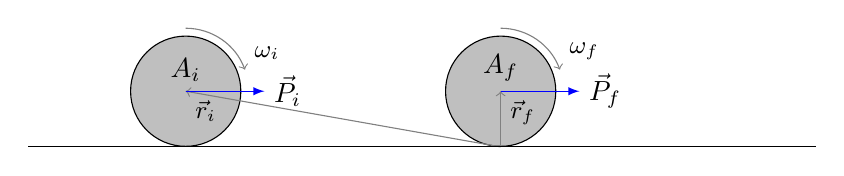
\begin{tikzpicture}[
    force/.style={>=latex,draw=blue,fill=blue},
    axis/.style={densely dashed,gray,font=\small},
    aux/.style={draw=gray,font=\small},
    M/.style={circle,draw,fill=lightgray,minimum size=1.4cm,thin},
    C/.style={draw,fill=lightgray,minimum size=1.4cm,thin},
    m/.style={rectangle,draw=black,fill=lightgray,minimum size=0.3cm,thin},
    plane/.style={draw=black,fill=blue!10},
    string/.style={draw=red, thick},
    pulley/.style={thick},
    tubo/.style={thick,draw=gray},
]
	 \node[M] at (0,0) (Ai) {};
	 \node at (Ai) [above] {$A_i$};
	 \node[M] at (4,0) (Af) {};
	 \node at (Af) [above] {$A_f$};
	  
	  \draw[aux,->] (Af.south)--(Ai.center) node [below right]{$\vec r_i$} ; % ri
	  \draw[aux,->] (Af.south)--(Af.center) node [below right]{$\vec r_f$} ; rf
	  \draw[aux,->] (0,0.8) arc (90:20:0.8) node [above right]{$\omega_i$};
	  \draw[aux,->] (4,0.8) arc (90:20:0.8) node [above right]{$\omega_f$};
	  \draw[plane] (-2,-0.7) --++(10,0);

	\draw[force,->] (Ai.center)--++(1,0) node [right]{$\vec P_i$}; %Pi
	\draw[force,->] (Af.center)--++(1,0) node [right]{$\vec P_f$}; %Pf
	%\node[axis] at (Af.south) [below] {$referencial$};
   	%\draw[force,->] (Ai.center) -- ++(0,-2) coordinate (fg) node [below right=-0.15cm] {$F_g$};


\end{tikzpicture}
\end{center}
$
\Delta \vec L=0 \quad \vec P_i=0 \quad \vec r_f \times \vec P_f=rmv_{cmf}$ , sem deslizamento final$\Rightarrow v_{cmf}=\omega_f r\\
$cf. alínea d), $\omega_i$ é igual ao $\omega_f$ das alíneas a) e b): $\omega_i=\frac{v_{cma,b}}{r}\\
\vec L_i=\vec r_i \times \cancel{\vec P_i}+I\omega_i=I\frac{v_{cma,b}}{r} \quad \vec L_f=\vec r_f \times \vec P_f + I\omega_f=rmv_{cmf} + I\frac{v_{cmf}}{r}\\
\\
\Leftrightarrow I\frac{v_{cma,b}}{r}=rmv_{cmf} + I\frac{v_{cmf}}{r}\Leftrightarrow \frac{2}{5}\cancel {mr}^{\bcancel 2}\frac{v_{cma,b}}{\bcancel r}=\cancel{rm}v_{cmf}+\frac{2}{5}\cancel{mr}^{\bcancel 2}\frac{v_{cmf}}{\bcancel r}\\
\\
\Leftrightarrow \boxed{v_{cmf}=\frac{2}{7}v_{cma,b}=1.511m/s}
\\\\
$
\hrule
\pagebreak

%									3a
\paragraph{3 a)} ~\\
$d\sin\theta=m\lambda$ \qquad 1ª ordem: $m = 1\\
\\
\boxed{d=\frac{\lambda}{\sin\theta}=1.183\mu m}\\\\
$
\hrule
%									3b
\paragraph{3 b)} ~\\
$d\sin\theta=m\lambda\\\\
$O máximo é visível se $\sin\theta \in [-1,1]$ (assume-se que o ecrã tem largura infinita)\\$
\\
\frac{m\lambda}{d} \in [-1,1] \Leftrightarrow -\frac{d}{\lambda}<m<\frac{d}{\lambda}\Leftrightarrow |m|<2.366\\
\\
\boxed{m=0,\pm 1, \pm 2 $: 5 máximos$}\\
$
\hrule
%									3ci
\paragraph{3 ci)}~\\
\begin{center}
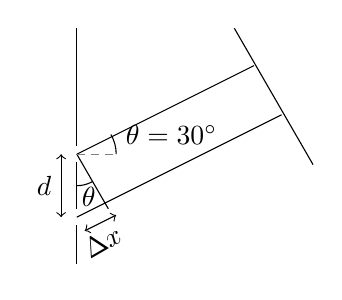
\begin{tikzpicture}[
    force/.style={>=latex,draw=blue,fill=blue},
    axis/.style={densely dashed,gray,font=\small},
    aux/.style={draw=gray,font=\small},
    M/.style={circle,draw,fill=lightgray,minimum size=1.4cm,thin},
    C/.style={draw,fill=lightgray,minimum size=1.4cm,thin},
    m/.style={rectangle,draw=black,fill=lightgray,minimum size=0.3cm,thin},
    plane/.style={draw=black,fill=blue!10},
    string/.style={draw=red, thick},
    pulley/.style={thick},
    tubo/.style={thick,draw=gray},
]
	{[plane]
	\draw (0,2)--(0,0.5);  % upper
	\draw (0,0.3)--(0,-0.3);  % islit
	\draw (0,-0.5)--(0,-1);  % lower
	\draw (2,2)--++(2*sin{30},-2*cos{30}); %target
		}
	{[force,->]
	\draw (0,0.4) {}  -- ++(2.25,sin{30}*2.25); % u beam
	\draw (0,-0.4) {}  -- ++(2.6,sin{30}*2.6); % l beam
	}
	{[aux]
	\draw (0,0.4) --++(0.8*sin{30},-0.8*cos{30}); %parallel
	\draw [axis ](0,0.4)--(0.5,0.4); %aux
	\node at (0.5,0.4) [above right]{$\theta=30^\circ$};
	\draw (0.5,0.4) arc (0:30:0.5); %upper angle
	\draw (0,0) arc (-90:-60:0.4); %lower
	\node at (0.15,0.1) [below]{$\theta$};
	\draw [<->](0+0.2*sin{30},-0.4-cos{30}*0.2)--++(0.8*sin{30},0.8*sin{30}*sin{30}); % delta x
	\node [rotate=30]at (0.2,-0.5) [below] {$\Delta x$};
	\draw [<->] (-0.2,0.4)--++(0,-0.8); % d
	\node at (-0.2,0) [left] {$d$};
	}
\end{tikzpicture}
\end{center}
~\\\\
$
\Delta x=d\sin\theta \qquad \boxed{\Delta \phi= \frac {2 \pi}{\lambda}\Delta x=7.433=2.366\pi}\\
$
\\
\hrule
%									3cii
\paragraph{3 cii)} ~\\\\
$
I=I_0\cos^2\frac{\phi}{2}\Leftrightarrow \cos^2\frac{\phi}{2}=\frac{1}{2}\Leftrightarrow\phi=90^\circ\\
\\
\Leftrightarrow\frac{2\pi}{\lambda}d\sin\theta=\frac{\pi}{2}\qquad \Leftrightarrow\sin\theta=0.0528\Leftrightarrow \boxed{\theta=6.07^\circ}\\
$
\\
\hrule
\pagebreak
%									3d
\paragraph{3 d)} ~\\
\begin{center}
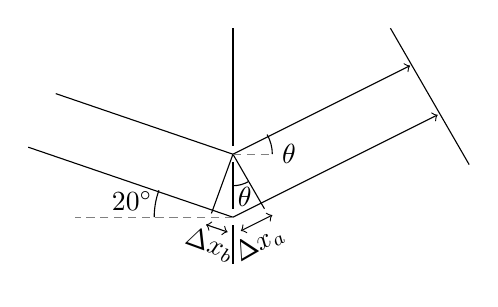
\begin{tikzpicture}[
    force/.style={>=latex,draw=blue,fill=blue},
    axis/.style={densely dashed,gray,font=\small},
    aux/.style={draw=gray,font=\small},
    M/.style={circle,draw,fill=lightgray,minimum size=1.4cm,thin},
    C/.style={draw,fill=lightgray,minimum size=1.4cm,thin},
    m/.style={rectangle,draw=black,fill=lightgray,minimum size=0.3cm,thin},
    plane/.style={draw=black,fill=blue!10},
    string/.style={draw=red, thick},
    pulley/.style={thick},
    tubo/.style={thick,draw=gray},
]
	{[plane]
	\draw (0,2)--(0,0.5);  % upper
	\draw (0,0.3)--(0,-0.3);  % islit
	\draw (0,-0.5)--(0,-1);  % lower
	\draw (2,2)--++(2*sin{30},-2*cos{30}); %target
		}
	{[force]
	\draw [->](0,0.4) {}  -- ++(2.25,sin{30}*2.25); % u beam
	\draw [->](0,-0.4) {}  -- ++(2.6,sin{30}*2.6); % l beam
	\draw (0,0.4) {}  -- ++(-2.25,sin{20}*2.25); % u beam
	\draw (0,-0.4) {}  -- ++(-2.6,sin{20}*2.6); % l beam
	}
	{[aux]
	\draw (0,0.4) --++(0.8*sin{30},-0.8*cos{30}); %parallel
	\draw [axis ](0,0.4)--(0.5,0.4); %aux
	\node at (0.5,0.4) [right]{$\theta$};
	\draw (0.5,0.4) arc (0:30:0.5); %upper angle
	\draw (0,0) arc (-90:-60:0.4); %lower
	\node at (0.15,0.1) [below]{$\theta$};
	\draw [<->](0+0.2*sin{30},-0.4-cos{30}*0.2)--++(0.8*sin{30},0.8*sin{30}*sin{30}); % delta xa
	\node [rotate=30]at (0.2,-0.5) [below] {$\Delta x_a$};
%	\draw [<->] (-0.2,0.4)--++(0,-0.8); % d
%	\node at (-0.2,0) [left] {$d$};
	\draw [axis](0,-0.4)--++(-2,0); %aux
	\draw (-1,-0.4) arc (180:160:1); %20 dg angle
	\node at (-0.9,-0.2) [left]{$20^\circ$};
	\draw (0,0.4) --++(-0.8*sin{20},-0.8*cos{20}); % left parallel
	\draw [<->](0-0.2*sin{20},-0.4-cos{20}*0.2)--++(-0.8*sin{20},0.8*sin{20}*sin{20}); % delta xb
	\node [rotate=-20]at (-0.2,-0.5) [below] {$\Delta x_b$};
	}

\end{tikzpicture}
\end{center}
As posições angulares dos máximos satisfarão:\\\\
$
\Delta x_{tot}=\Delta x_a+\Delta x_b =d\sin\theta+d\sin20=m\lambda\\
\\
\Leftrightarrow\boxed{\theta=\arcsin\left (\frac{m\lambda}{d}-\sin20 \right )}\\
\\
$
\begin{align*}
	m &\quad \theta\\
	-2 &\quad  -\\
	-1 &\quad -49.88^\circ\\
	0 &\quad -20^\circ\\
	1 &\quad 4.63^\circ\\
	2 &\quad 30.22^\circ\\
	3 &\quad 67.81^\circ\\
	4 &\quad -
\end{align*}
\hrule
%\includepdf[fitpaper=true, pages=2-3]{/home/halves/Dropbox/work/MOAero2019/scan.pdf}
%\theta=\arcsin(\frac{m\lambda}{d})
%%									3a
%\paragraph{3a)} ~\\
%\\
%\begin{minipage}[t]{0.3\textwidth}
%$
%x_1=17t\\
%x_2=14-3t\\
%$
%\end{minipage}
%%second column
%\begin{minipage}[t]{0.3\textwidth}
%$
%\dot x_1=17\\
%\dot x_2=3\\
%$
%\end{minipage}
%\\
%$
%x_{CM}(t)=\frac{2\times 17t+5\times (3t+14)}{2+5}=7t+10 \qquad \dot x_{CM}=7 m/s\\
%$
%\\
%\hrule
%%									3b
%\paragraph{3b)} ~\\
%\\
%No ponto de compressão máxima $v_1=v_2=v_{CM}=7m/s\\
%\\
%\begin{minipage}[t]{0.6\textwidth}
%$
%T_i=\frac{1}{2}(2 \times 17^2+5 \times 3^2)=\frac{623}{2}\\
%\\
%T_{comp.max}=\frac{1}{2}(2+5)\times7^2=\frac{343}{2}\\
%$
%\end{minipage}
%\begin{minipage}[t]{0.3\textwidth}
%$
%T_i+\cancel{V_i}=T+V\\
%$
%\end{minipage}
%$
%\\
%$
%V=\frac{kx^2}{2}=T_i-T_{comp.max}\\
%\\
%\Leftrightarrow \frac{623}{2}-\frac{343}{2}=\frac{kx^2}{2} \Leftrightarrow x_{max}=\sqrt{\frac{280}{4480}}=0.25m\\
%$
%\\
%\hrule
%%									3c
%\paragraph{3c)} ~\\
%\\
%Trata-se duma colisão elástica e portanto $\Delta p =0$ e $\Delta E_c=0$:\\
%\\
%$2 \times 17+5\times3=2\times v_1+5 \times v_2 \Leftrightarrow v_1=\frac{49-5v_2}{2}\\$
%e\\
%$2 \times 17^2+5\times 3^2=2 \times v_1^2+5 \times v_2^2 \Leftrightarrow 623=(\frac{49-5v_2}{2})^2+5v_2^2 \\
%\\
%\Leftrightarrow 35v^2_ 2+490v_ 2+1155=0\\
%\\
%\Rightarrow v_ 2=\frac{490\pm 280}{70}=3 \vee \boxed{11} \Rightarrow v_1=17 \vee \boxed{-3}$
%
%

\end{document}